% !TEX encoding = UTF-8 Unicode
\documentclass{article}
\usepackage[utf8]{inputenc}
\usepackage{amsmath,amssymb}
\usepackage{paralist}
\usepackage{color}
\usepackage[detect-weight=true, binary-units=true]{siunitx}
\usepackage{pgfplots}
\usepackage{authblk}
\usepackage{url}
\usepackage{multirow}
\usepackage{booktabs}

%\usepackage{biblatex}
\usepackage[backend=biber]{biblatex}
\addbibresource {bibliography.bib}

\title{Machine Learning and Data Mining progetto:\\Black Friday}
\author{Michele Belletti}

\date{Corso AA 2019-2020}



\begin{document}

\maketitle



\section{Identificazione del problema}
Data l'evoluzione esponenziale dei negozi online bisogna trovare soluzioni per rendere competitiva una piattaforma rispetto ad un altra. Le idee proposte sono una stima delle vendite e una stima della categoria che all'utente potrebbe interessare. Queste stime ci permettono di avere una conoscenza a priori del volume di vendita di tale piattaforma e anche ci permette di gestire al meglio le vendite potendo così ricavare un utile maggiore.

\section{Indici di valutazione e prestazione}
Il metodo che andremo ad utilizzare per la valutazione del modello sarà basata sulla percentuale di successo della predizione e del valore dell'errore RSME.
Il rapporto fra i dati utilizzati per la creazione della modello e i dati utilizzati per la realizzazione della verifica saranno rispettivamente l'80 \% dei dati a disposizione per il primo mentre il rimanente 20\% per la verifica.

\section{Soluzione Proposta}
Supponendo il problema  lineare, perciò andremo a risolvere un problema di regressione. Gli algoritmi che andremo ad utilizzare sono: regressione lineare, decision tree regression e random forest regression.

Data la presenza di valori non definiti (NaN) nella categoria dei prodotti 2 e 3, opteremo per 2 diversi approcci:
\begin{itemize}
\item elimineremo le categorie 2 e 3, ipotizzando che siano sottocategorie della prima, cioè categorie meno importanti per descrive il prodotto;
\item assegneremo un valore scorrelato al sistema che descrivono, in modo che non facciano variare la stima, in più aggiungeremo dei dati che ci permetteranno di stimare più correttamente.
\end{itemize}

Poi andremo a determinare un algoritmo per la determinazione della categoria migliore di prodotti da consigliare ad un utente. Tale sistema sarà costruito in modo generale in modo da funzionare in qualsiasi condizione, cioè sia utenti già inscritti che utenti nuovi.

\section{Valutazione sperimentale}
Inizieremo ora a creare il sistema in base alle ipotesi sopra descritte.

\subsection{Data}
La prima cosa che si deve fare per la descrizione e la realizzazione di un modello è l'analisi dei dati a disposizione.

I dati a nostra disposizione sono gli ordini effettuati durante il Black Friday e sono contenuti in un file csv avente le seguenti informazioni:
\begin{itemize}
\item L'utente attraverso il suo codice identificativo UserID;
\item Il prodotto che l'utente ha comprato ProductID;
\item L'eta dell'utente: Gender Age (valore che viene diviso ad intervalli di età 0-17, 18-25, 26-35, 36-45, 46-55, 55+;
\item Il tipo di occupazione: Occupation (21 diverse occupazioni);
\item La categoria della città:  CityCategory (A,B,C che si suppone dipendano dalle dimensioni);
\item Quanti anni sono passati da quando vive in quella città: StayInCurrentCityYears (0, 1, 2, 3, 4+);
\item Stato civile: MaritalStatus;
\item Le categorie del prodotto comprato: ProductCategory1, ProductCategory2, ProductCategory3;
\item E la quantità dei soldi spesi: Purchase.
\end{itemize}

Ora analizzeremo i dati in funzione del numero di ordini (grafici 1-2-3-4-5-6):

\begin{figure}[htp!]
\centering
\frame{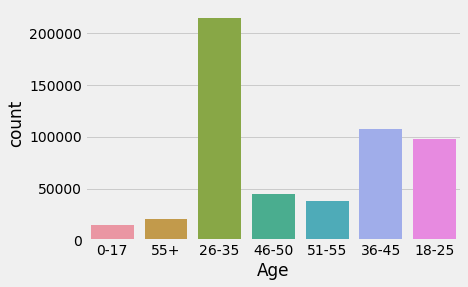
\includegraphics[width=0.3\textwidth]{ima/age_purchase.png}}
\frame{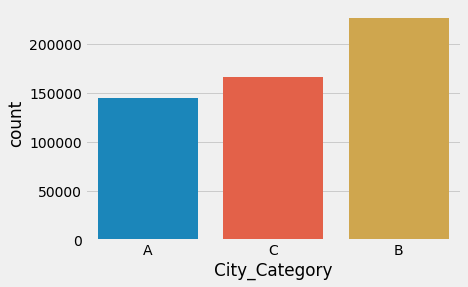
\includegraphics[width=0.3\textwidth]{ima/city_purchase.png}}
\frame{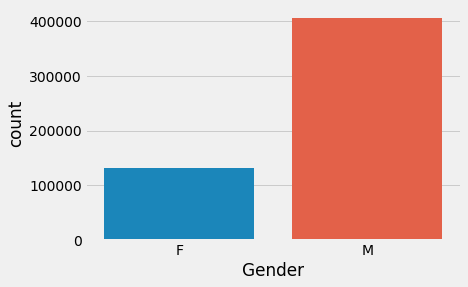
\includegraphics[width=0.3\textwidth]{ima/men_female_purchase.png}}
\frame{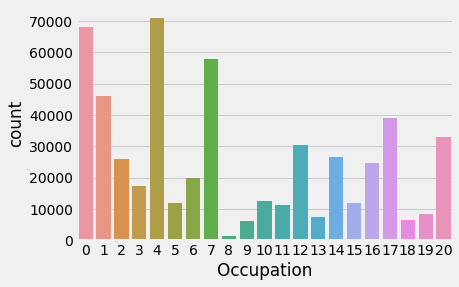
\includegraphics[width=0.3\textwidth]{ima/occupation_purchase.png}}
\frame{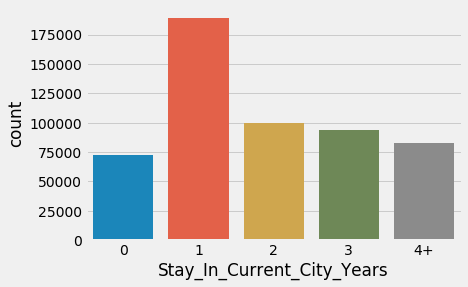
\includegraphics[width=0.3\textwidth]{ima/time_in_city_purchase.png}}
\frame{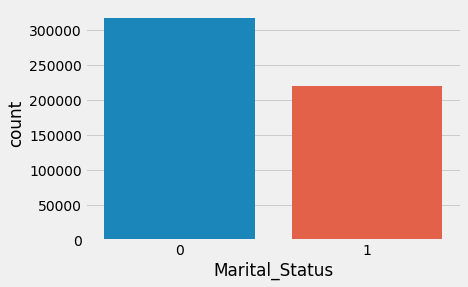
\includegraphics[width=0.3\textwidth]{ima/marital.png}}
%%\caption{...}
%%\abel{fig:...}
\end{figure}

Si vede che gli ordini sono fatti principalmente da:
\begin{itemize}
\item persone di età tra i 26-35 anni, età nella quale si è più inclini ad utilizzare i mezzi della rete per acquistare i prodotti e si ha più disponibilità economica;
\item le città di categoria B;
\item i maschi e persone single;
\item le persone con un occupazione di tipo 0, 4 e 7;
\item e le persone che sono da circa un anno in città.
\end{itemize}

Analizzando la matrice di correlazione che esprime il grado di dipendenza tra due variabili si vede che non c'è una vera correlazione tra i dati a disposizione e il valore del purchase.
Questo vale anche per il caso di voler suggerire una tipologia di prodotto, tranne che per le sottocategorie dove c'è una buona correlazione, ma non conoscendo neanche la prima categoria non possiamo neanche conoscere le sottocategorie il che ci porta a eliminarle nel calcolo della stima.

\begin{figure}[htp!]
\centering
\frame{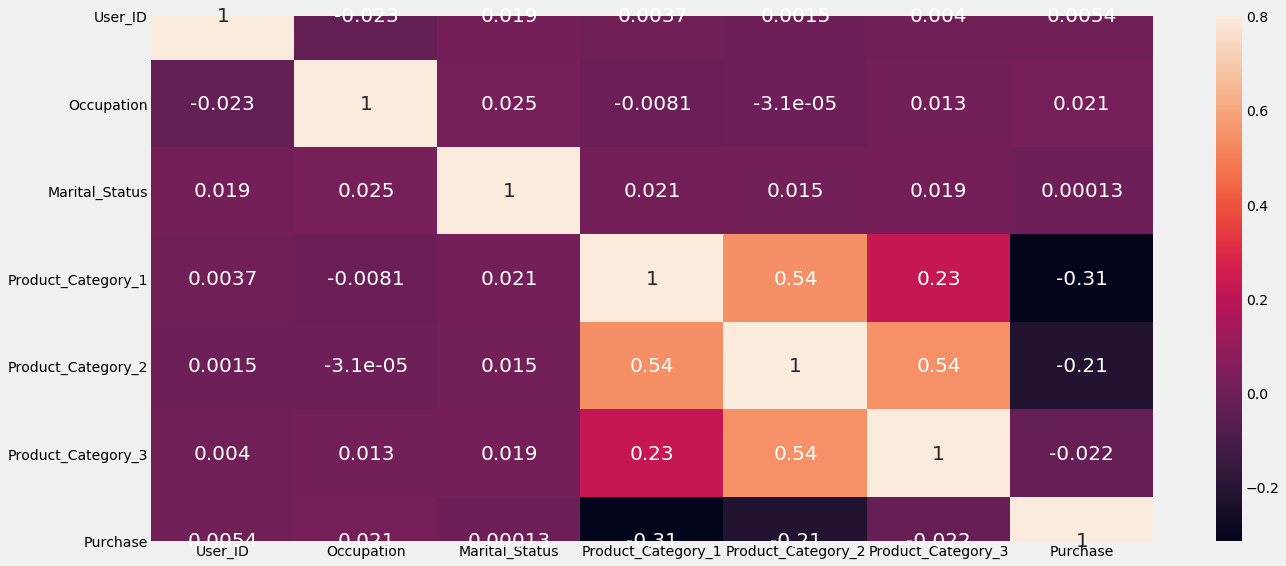
\includegraphics[width=0.8\textwidth]{ima/crosscorrelazione.png}}
%%\caption{...}
%%\abel{fig:...}in
\end{figure}

Andiamo ora ad analizzare le variabili indipendenti rispetto alla variabile Purchase che vogliamo prevedere:
\begin{figure}[htp!]
\centering
\frame{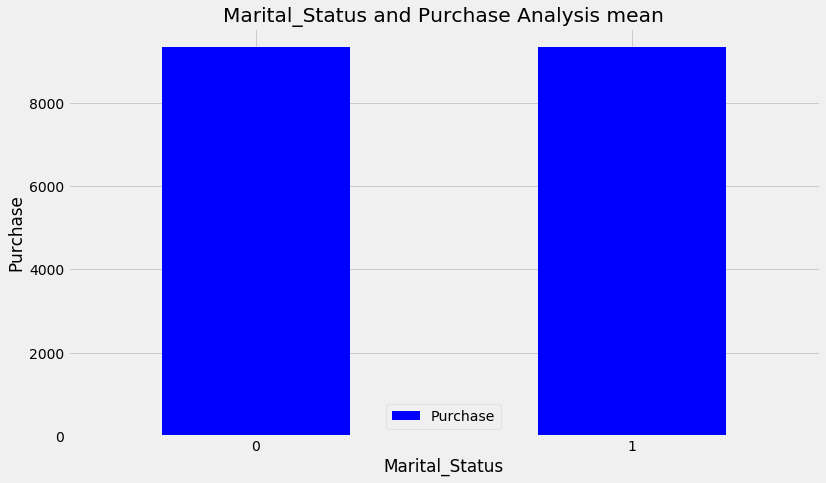
\includegraphics[width=0.3\textwidth]{ima/mean_marital_purc.png}}
\frame{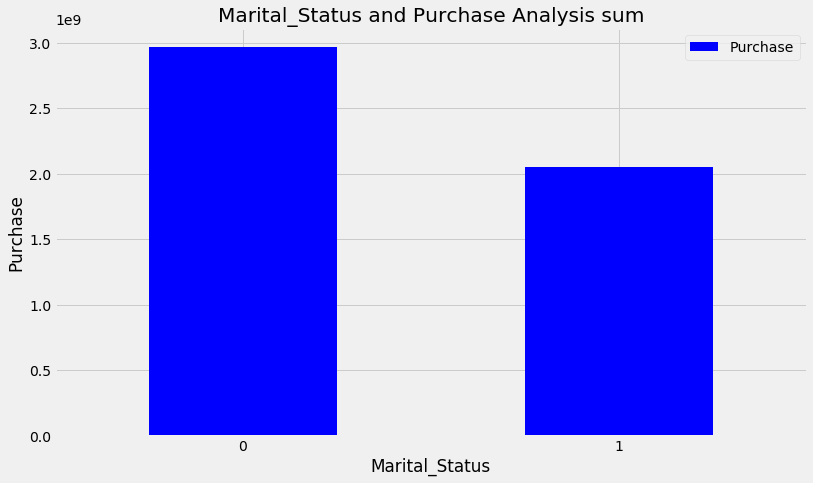
\includegraphics[width=0.3\textwidth]{ima/sum_marital.png}}
%%\caption{...}
%%\abel{fig:...}
\end{figure}

Si ha che i grafici valutati con la media non differiscono tra i valori assegnati, l'unico grafico che non è uniforme in tal caso è quello che definisce la quantità del prodotto rispetto alla categoria.
Dato che la media non appare come dato importante ma la loro quantità si, per migliorare la stima andremo anche a tener conto della sua quantità. Questa aggiunta permette di avere una stima migliore, come vedremo in seguito.

Invece questo cambia nel caso della categoria del prodotto(grafici 9-10):
\begin{figure}[htp!]
\centering
\frame{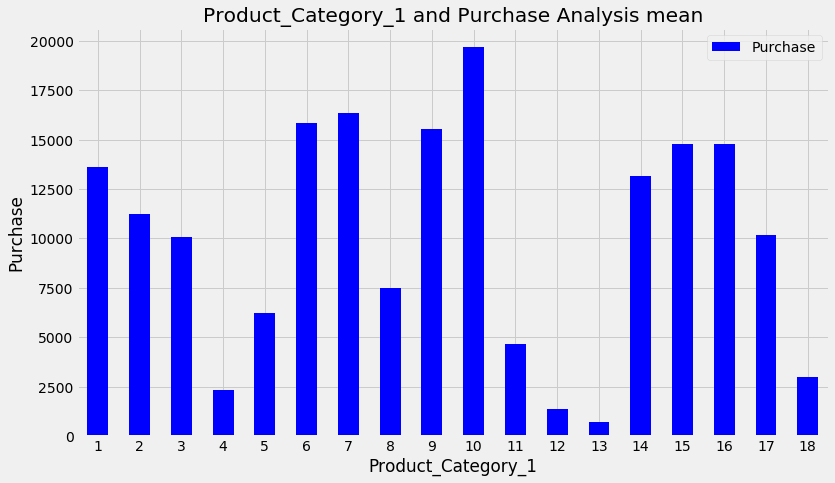
\includegraphics[width=0.3\textwidth]{ima/sum_cat_pur.png}}
\frame{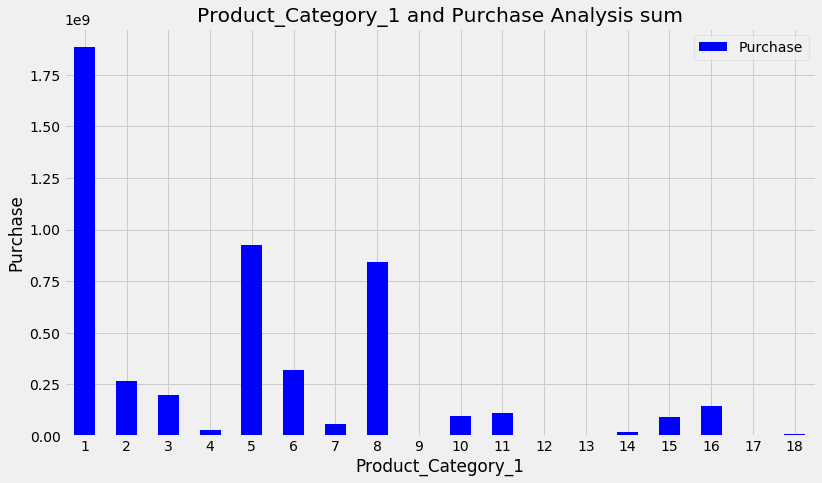
\includegraphics[width=0.3\textwidth]{ima/cate_purc.png}}
%%\caption{...}
%%\abel{fig:...}
\end{figure}

Analizzati i dati andremo a realizzare il modello:
 

\subsection{Procedimento}

I dati verranno tutti riportati in codice binario in modo che gli algoritmi possano gestirlo.

Come definito prima andremo ad utilizzare i seguenti algoritmi con le seguenti impostazioni:
\begin{itemize}
\item linear regression : normalizzazione attiva;
\item DecisionTreeRegressor : max\_ depth=15, min\_ samples\_ leaf=100;
\item Random Forest: max\_ depth=8, min\_ samples\_ leaf=150.
\end{itemize}

Adesso valuteremo questi 3 algoritmi con i diversi metodi proposti:
il primo metodo utilizzato per predirre la quanti di soldi spesi sarà basato sull'eliminazione dei dati delle categorie dei prodotti 2 e 3. Elimineremo anche l'identificazione dell'utente perchè non influisce sulla predizione della spesa, così come il codice del prodotto. Queste due ultime eliminazioni permettono di stimare meglio l'aggiunta di un nuovo utente però peggiora la stima per un vecchio utente, dato che non c'è correlazione tra i suoi vecchi ordini. I risultati sono riportati nella prima tabella nella sezione risultati e discussione.

Il secondo metodo utilizza anche i dati della categoria 2 e 3, naturalmente si avrà una stima migliore dato che aggiungo altri dettagli all'ordine(13\%). In più aggiungo anche il numero totale degli ordini con quel valore di eta, occupazione, tipo di categoria e identificazione del prodotto. Tali dati aggiuntivi permette di stimare meglio il risultato. I risultati sono riportati nella seconda tabella.


Fatto questo possiamo definire un sistema di raccomandazione per l'utente. Utilizzeremo i dati per l'ultimo metodo ed elimineremo ogni conoscenza rispetto alla categoria del prodotto. I risultati sono riportati nella terza tabella:



\subsection{Risultati e discussione}
I risultati sono i seguenti: usando \cite{scikit-learn}

Prima tabella:

\begin{tabular}{|p{0.2\textwidth}|p{0.2\textwidth}|p{0.2\textwidth}|p{0.2\textwidth}|}
\hline
Algoritmi &Linear Regression          & Decision tree regression         &random forest regression      \\
\hline
Risultati & 10.28\%            & 63.90\%     & 63.00\%          \\
\hline
RMSE     & 4708     & 2954                & 3008           \\
\hline
\end{tabular}

Seconda tabella:

\begin{tabular}{|p{0.2\textwidth}|p{0.1\textwidth}|p{0.2\textwidth}|p{0.2\textwidth}|}
\hline
Algoritmi &Linear Regression          & Decision Tree Regression         &Random Forest Regression      \\
\hline
Risultati &24.00\%            & 70.16\%    & 68.22\%          \\
\hline
RMSE &4344 &2685 &2802\\
\hline
\end{tabular}

Si ottiene che il migliore risultato è il secondo caso, cioè con i dati aggiuntivi definiti  prima. In più l'algoritmo  Decision tree regression ottiene una migliore predizione e un minore RMSE.

Terza tabella: 

\begin{tabular}{|p{0.2\textwidth}|p{0.2\textwidth}|p{0.2\textwidth}|p{0.2\textwidth}|}
\hline
Algoritmi &Linear Regression          & Decision tree Classifier         &random forest Classifier      \\
\hline
Risultati & 10.71\%           & 86.79\%    & 82.72\%          \\
\hline
RMSE &3.552 &2.56 &2.807\\
\hline
\end{tabular}

Questi risultati dimostrano che il processo così costruito non fornisce una stima buona del tipo di prodotto consigliato. Per migliorare la stima si deve tener conto dell'utente, il che può essere fatto in due casi:
\begin{itemize}
\item l'aggiunta dell'utente all'algoritmo complessivo, il che porta ad avere un alto tempo di calcolo e il problema  di quando si aggiunge un nuovo utente;
\item oppure generare diversi algoritmi, uno per utente, che permetterà così di descrivere meglio le sue preferenze in più ridurrà il tempo di stima ma aumenta lo spazio in memoria perchè l'algorimo è definito in modo univoco.
\end{itemize}
Il codice è disponibile a \url{https://github.com/michbelle/Machine_learning_project.git}

\nocite{*}
\printbibliography[title=Bibliografia]{}


\end{document}
